\section{\label{sec:clas.tagr}Radiator and Electron Tagger (\abbr{TAG})}

\abbr{CLAS} can use the electron beam as it is delivered from \abbr{CEBAF} by sending it directly to the target. There are a number of experiments which use the electron beam in this fasion. For example, a series of experiments called Deeply Virtual Compton Scattering (\abbr{DVCS}\label{abbr:dvcs}) is currently on-going\cite{avakian2010}, however, the detector is also capable of producing a beam of \emph{real photons} by passing the electrons through a radiator. This causes the electron beam to emit photons via \emph{bremsstrahlung} radiation. The electrons are subsequently bent out of the way by a dipole magnet and the photons continue on to the target. This is known as \emph{photon running} with \abbr{CLAS} and a typical reaction studied looks like
\begin{equation}
	\mathrm{\gamma p \rightarrow p \pi^{+}  \pi^{-}}
\end{equation}

Knowing the incoming electron's energy, the photon's energy can be determined by measuring the momentum of the electron after it has emitted the photon. The electrons are then bent by a dipole magnet and the energy and timing of individual electrons are recorded by the tagger counters\cite{clas.tagger} (\abbr{TAG}) while the photons continue to the target.  In the \g12 experiment, there were usually many ``hits'' in the tagger for each event. Normally, the one associated with the photon that caused the event could be obtained by a timing coincidence with the tracks, though there are cases when this photon is ambiguous as discussed in Sec.~\ref{sec:analysis.beam}.

The \g12 experiment was a \emph{photon run} with an electron beam energy of 5.7~GeV meaning that the tagged photon energy ranged from 1.2 to 5.4~GeV. The radiator used was a gold foil $10^{-4}$~radiation lengths thick. The photons passed through a 6.2~mm diameter collimator 527~cm before they entered the target which had a radius of 2~cm.

\begin{figure}\begin{center}
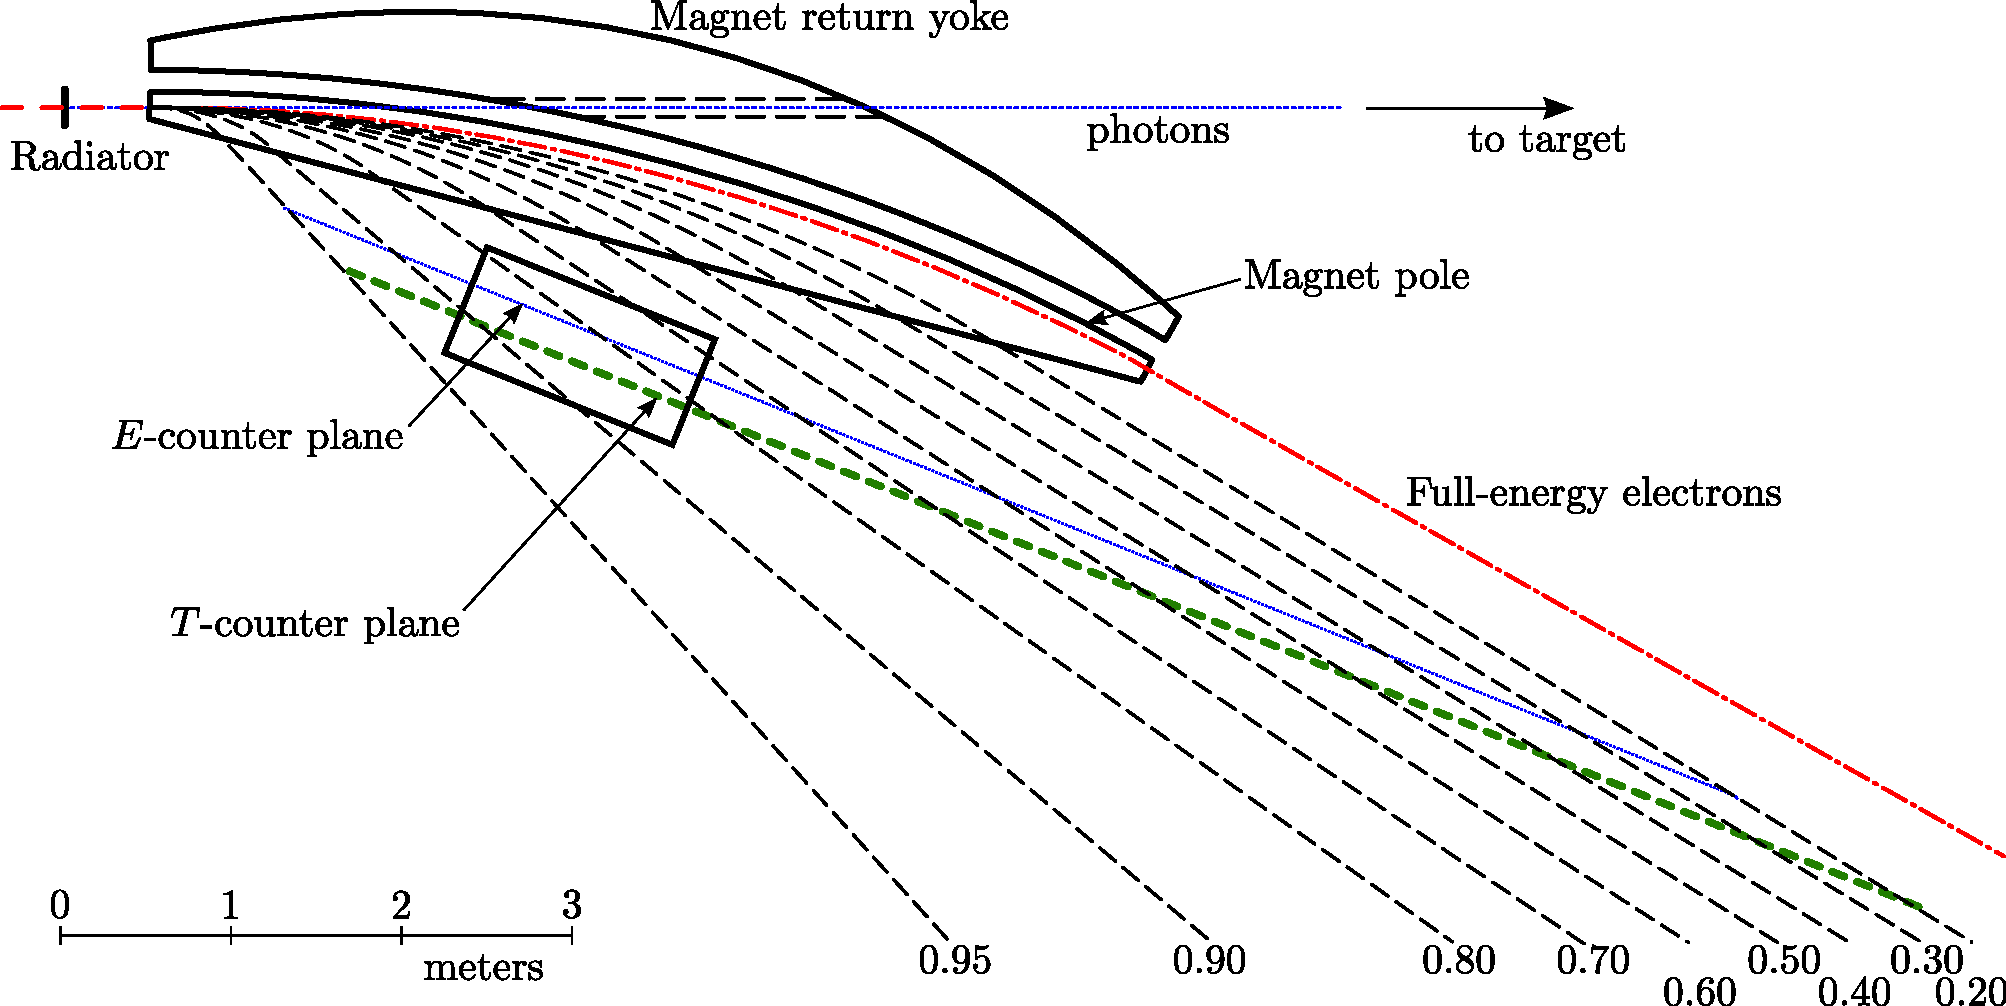
\includegraphics[width=1.1\figwidth]{\grpath/hall-b/tagger_energies.pdf}
\caption[Tagger Schematic - Energies]{\label{fig:jlab.tagr.energies}Scale drawing of the photon tagger system. The electron beam enters from the left and passes through the radiator where a few electrons \emph{bremsstrahl}. The electrons that don't, follow the dash-dot red line to the tagger beam-dump. The electrons that lose energy (black dashed lines) get directed by the dipole magnet to the $E$-counter and $T$-counter planes and the photons continue to the target. The tagging range for the photons is 20\% to 95\% of the beam energy incident on the radiator. The rectangle around the $E$ and $T$-counter planes outlines the expanded view shown in Fig.~\ref{fig:jlab.tagr.paddles}.}
\end{center}\end{figure}

\begin{figure}\begin{center}
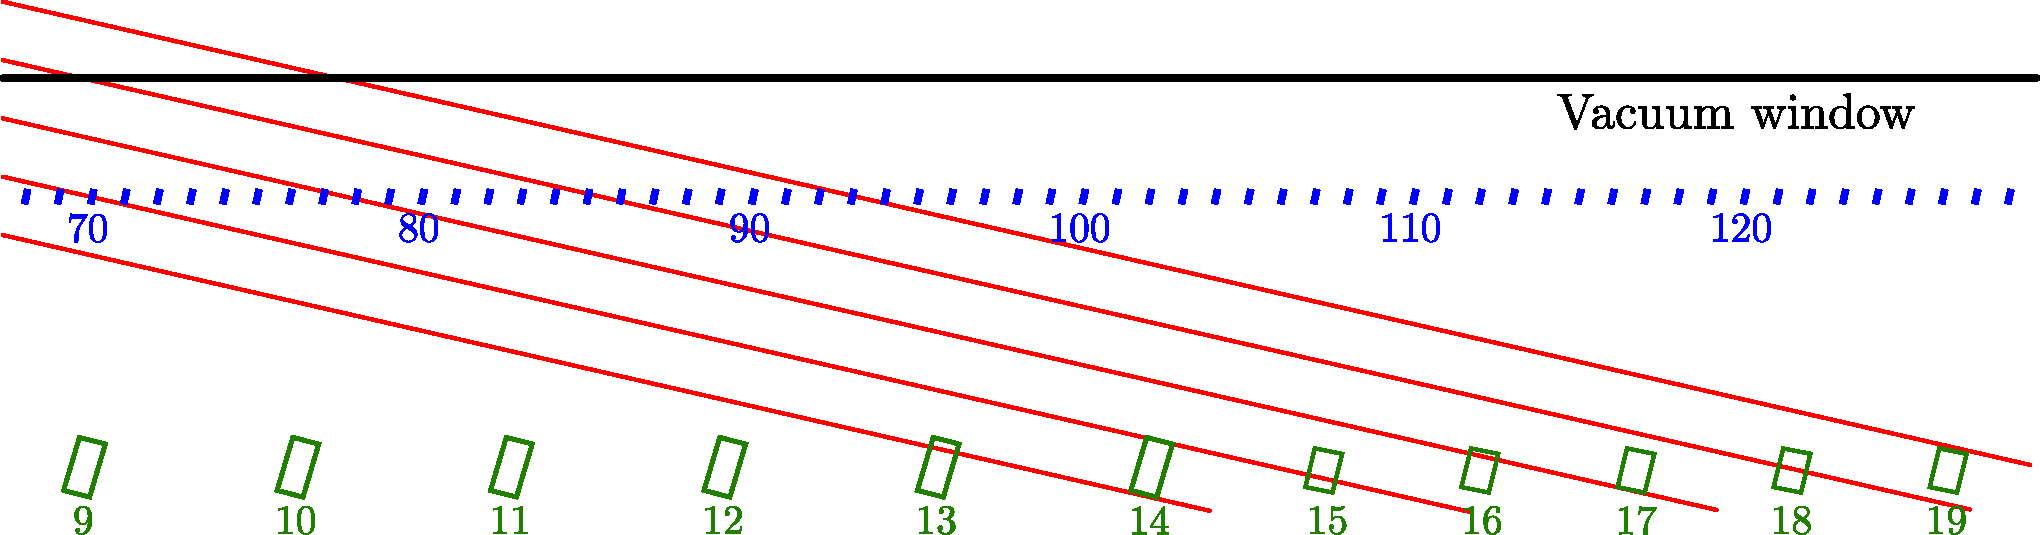
\includegraphics[width=1.1\figwidth]{\grpath/hall-b/tagger_paddles.pdf}
\caption[Tagger Schematic - Paddles]{\label{fig:jlab.tagr.paddles}{\coloronline}Scale drawing of the $E$-counters (upper plane of counters in blue) and the $T$-counters (lower plane of counters in green) showing examples of incident electrons (red lines) entering from the upper left. This view corresponds to the rectangle in Fig.~\ref{fig:jlab.tagr.energies}. Notice how both sets of counters overlap, providing fine segmentation and hermetic coverage. The $T$-counters each consist of two \abbr{PMT}s (\emph{left} and \emph{right}) which are averaged together to obtain the time of the hit. The resolution produced by this setup, crucial for missing mass calculations, is determined by the size and overlap of the $E$-counters as discussed in Sec.~\ref{sec:data.calib.systems}.}
\end{center}\end{figure}
